\documentclass{article}
\usepackage[english]{babel}
\usepackage[margin=0.5in]{geometry}
\usepackage{longtable}
\usepackage{tabu}
\usepackage{graphicx}
\usepackage{enumitem}
\usepackage{import}
\usepackage{titlesec}
%\newcommand{\herpname}[1]{\begin{center} \Large{\textbf{#1}} \end{center}}
%\titleformat*{\section}{\Large\bfseries}

\begin{document}
\tableofcontents
\pagebreak
\section{Crocodylia}

\subsection{Crocodylidae -- Crocodiles}
\begin{center}
\begin{longtabu} to \textwidth {| | p{3.5cm} | X | |}
	\hline
	Taxonomy/Ancestry & 
	\begin{itemize}[noitemsep]
		\item subfamilies -- crocodylinae, mekosuchinae (ex.), tomistominae
		\item \textbf{tomistominae} -- false gharial; genetic evidence suggests they are closer to the gharials so they may be reclassified into the Gavialidae family
		\item 3 extant genera; 16-17 species
		\item Ancient Greek = ``lizard of the Nile"
		\item separated from other crocodilians during Eocene epoch 55 million years ago
		\item closest living relatives are birds
	\end{itemize}
	\\
	\hline
	Size & 
	5-20 ft (1.5-6.1 m)
	
	weigh up to 2000 lb (900 kg)
	
	juveniles 20 cm (7.9 in)
	\\
	\hline
	Color & \\
	\hline
	Anatomy & 
	\begin{itemize}[noitemsep]
		\item diapsid skull
		\item dorsal scales backed by osteoderms from heavy armor plating on neck and back
		\item tail strongly muscled and flattened for swimming
		\item aquatic adaptations
			\begin{itemize}[noitemsep]
			\item nostril/ear valves
			\item nictitating membrane to cover eye
			\item glottal valve in throat
			\item able to concentrate and excrete salt; salt glands on tongue filter salt to allow for survival in saltwater environments
			\end{itemize}
		\item webbing on toes of the hind feet speeds swimming + gives advantage on dry land
		\item cerebral cortex w/ 4-chambered heart
		\item slit pupils w/ tapetum lucidum
		\item teeth are replaced throughout lifespan
		\item poikilothermic + ectothermic
		\item live 70-80 yrs
		\item distinguishing from alligators
			\begin{itemize}[noitemsep]
			\item narrower + longer heads
			\item v-shaped snouts
			\item lower teeth protrude when mouth closed
			\item large 4th tooth visible
			\item salt glands = saltwater habitat
			\item sensory pits all over body
			\item jagged fringe on hind legs + feet
			\item more aggressive + dangerous
			\end{itemize}
	\end{itemize}
	\\	
	\hline
	Dimorphism & 
	males grow larger + faster
	\\
	\hline
	Behavior & 
	\begin{itemize}[noitemsep]
		\item nocturnal hunter-scavengers
		\item often bask on shoreline
		\item aestivate during drought or arid conditions
		\item adult males bellow, growl, or hiss for dominance
		\item hatchlings grunt, squawk, communicate thru ultrasound
	\end{itemize}
	\\
	\hline
	Habitat & 
	Hill streams, large rivers, marshes, ponds, lakes, canals, reservoirs, saline habitats (i.e. mangrove creeks/saltpans)
	
	Deep water = safety + drought resistance but some species live in places where water regularly dries (Crocodylus suchus) by living in deep tunnels or caves; drought can also force species to move inland 
	\\
	\hline
	Distribution & 
	tropical + subtropical regions in Africa, Asia, Americas, Australia
	\\
	\hline
	Feeding Ecology &
	\begin{itemize}[noitemsep]
		\item opportunistic apex of the food chain
		\item young are agile + can jump to eat dragonflies, termites, spiders, other insects
		\item adolescents begin to feed on crabs, fish, frogs, reptiles, birds, + mammals
		\item scavenge for carrion
		\item teeth/jaws designed for seizing, tearing, + crushing rather than chewing
		\item some species have narrow jaws + sharp teeth to hunt fish
		\item	Sensory pores in or around mouth to help detect prey
		\item	Some species herd fish to shore w/ their bodies, often communally
		\item	Control predators of commercially important fish + help maintain cleanliness as scavengers
	\end{itemize}
	 \\
	\hline
	Reproductive Biology & 
	\begin{itemize}[noitemsep]
		\item males defend territories + compete for mates
		\item fixed breeding seasons where males mate w/ multiple females
		\item females lay eggs 40-70 days after mating; incubation period depends on nest temp (avg. 60-90 days)
			\begin{itemize}[noitemsep]
			\item higher temperatures = male, lower temperatures = female
			\item \textbf{hole-diggers} -- females dig in sand, earth, or gravel embankments above the hindwater line w/ clawed hind-limbs; eggs emerge lubricated + hatch with the wet season
			\item \textbf{mound-nesters} -- females gather vegetation, soil, or compost  and digs a hole on top to lay eggs; eggs are laid at the start of the wet season and hatch when the water is highest
			\end{itemize}
		\item females, sometimes males, guard nest during incubation
		\item young call w/ quacking grunts when ready to emerge so parents release young and carry to water
		\item young are cared for in creche formation w/ parents guarding young for 90 days
		\item adults are conditioned to respond to young distress calls
		\item mortality rate = 90\% due to predators
	\end{itemize}
	\\
	\hline
	Conservation Status &
	populations are reduced due to overhunting (for skin) and habitat loss due to human industrialization. sustainable-use programs responsible for recovery and continued survival of species like Nile, saltwater, and New Guinea crocodiles. 3 CR; 2 EN; 3 VU; 1 CD; 1 DD. 
	
	In Ancient Egypt (Sobek and Taweret), Hinduism (Varuna, Ganga, Yamuna, Goa), Aztec (Cipactli)
	 \\
	\hline 
\end{longtabu}
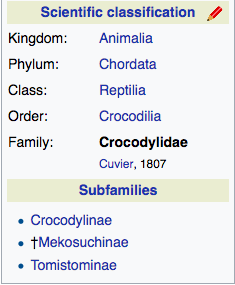
\includegraphics[scale=0.75]{crocodylia/crocodylidae/crocodylidae.png}
\end{center}
\pagebreak

\subsection{Alligatoridae --- Alligators}
\begin{center}
\begin{longtabu} to \textwidth {| | p{3.5cm} | X | |}

	\hline
	Taxonomy/Ancestry &
	subfamilies:
	\begin{itemize}[noitemsep]
		\item \textbf{alligatorinae} -- true alligators; only 1 of 10 genera currently extant; represented today by \emph{A. mississippiensis} in US and \emph{A. Sinesis} in China
		\item \textbf{caimaninae} -- caimans in C. and S. America
	\end{itemize}
	
	\begin{center} 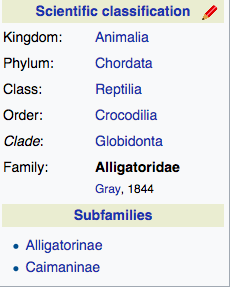
\includegraphics[scale=0.5]{crocodylia/alligatoridae/taxonomy} \end{center}
	 \\
	\hline
	Size & 
	alligator: 5-20 ft (1.5-6.1 m)
	
	caiman: average maximum weight of 6 to 40 kg (13 to 88 lb) depending on species, with the exception of the black caiman (Melanosuchus niger), which can grow more than 5 m (16 ft) in length and weigh up to 1,100 kg (2,400 lb). The average length for most of the other caiman species is about 2 to 2.5 m (6.6 to 8.2 ft) long. largest species = black caiman, smallest = Cuvier's dwarf.
	\\
	\hline
	Color &
	
	 \\
	\hline
	Anatomy &
	\begin{itemize}[noitemsep]
		\item diapsid skull
		\item armored w/ osteoderms and large scales that do not overlap
		\item forelimbs are smaller and weaker with 5 partially-webbed toes
		\item distinguishing from crocodiles:
			\begin{itemize}[noitemsep]
				\item wider, shorter heads w/ more obtuse snouts
				\item 4th enlarged underjaw tooth fits into pit in upper jaw --> no teeth visible when mouth closed
				\item no jagged fringe on hind legs + feet
				\item sensory pits appear only on snout and face, not neck and body
				\item toes of hind feet webbed not more than halfway to tips
				\item intolerant to salinity
				\item generally less aggressive and dangerous
				\item partake in foliage and fruit in addition to fish and meat
			\end{itemize}
		\item caiman characteristics:
			\begin{itemize}[noitemsep]
				\item no bony septum b/w nostrils
				\item ventral armour composed of overlapping bony scutes formed from two parts united by a suture
				\item longer, more slender, teeth than those possessed by alligators. The calcium rivets on its scales make their hides stiffer, and thus less valuable, than those of alligators and crocodiles.
			\end{itemize}
	\end{itemize}
				
	 \\
	\hline
	Dimorphism & 
	males larger and grow faster.
	
	\\
	\hline
	Behavior & 
	\begin{itemize}[noitemsep]
		\item ectotherms basking on shoreline
		\item float on surface of water
		\item become more subdued as temperatures drop but do not hibernate, making use of burrows in the winter months
		\item live in groups w/ dominance hierarchies. the highest-ranking individuals assert dominance through ritualized behaviors such as vocalizations and slapping the water with their heads.
		\item \textbf{high walk}: 4-limbed forward motion used for overland travel w/ belly up from the ground
		\item alligator holes in the wetlands increase plant diversity and provide habitats for other animals during droughts
		
	\end{itemize}
	\\
	\hline
	Habitat & 
	lakes, slow-moving streams/rivers, rivers, swamps, marshes, occasionally roadside ditches. freshwater sites w/ slow or still waters. often inhabit heavily-vegetated areas w/ muddy or murky water.
	\\
	\hline
	Distribution & 
	a New World group w/ habitats in Central-Northern S. America; parts of southern and western Central America and Mexico; SE United States; eastern China.
	\\
	\hline
	Feeding Ecology & 
	\begin{itemize}[noitemsep]
		\item opportunistic scavenger-hunters
		\item juveniles mainly eat snails and other invertebrates
		\item Typical adult diet = fish, small mammals, other reptiles (including smaller alligatorids), and birds, occasionally continuing to eat snails/invertebrates
		\item Predation typically occurs among eggs and hatchlings
		\item Racoons, coati, foxes, skunks, and other mammals, snakes, and various raptors, can raid nests or take hatchlings
		\item occasional cannibalism, but rare
		\item larger alligators help control coypu population
	\end{itemize}
	\\
	\hline
	Reproductive Biology & 
	\begin{itemize}[noitemsep]
		\item spring reproductive season
		\item courtship rituals thru loud bellowing choruses, vibrations of the male trunk
		\item use vegetables to construct nest mounds
		\item 12-60 eggs depending on species
		\item egg-laying once a year in midsummer, w/ eclosion 1-2 months afterward
		\item females respond to noises from eggs and assist offspring. offspring also use egg teeth for eclosion.
		\item females remain w/ offspring for up to 1 year.
		\item TSD is associated w/ several species, such as American alligator and common caimans. <88degF/31degC = female; >90degF/32degC = male. natural sex ratio of 5:1 female:male.
		\item Muja = oldest known in Serbia
	\end{itemize}
	\\
	\hline
	Conservation Status & 
	\begin{itemize}[noitemsep]
		\item raised commercially for their meat and skin
		\item ecotourism industry
		\item in Louisiana, heavy grazing by coypu and muskrat are damaging coastal wetlands
		\item Chinese alligator critically endangered; Louisiana and Florida zoos have some in captivity they are trying to preserve
	\end{itemize}
	\\
	\hline
\end{longtabu}
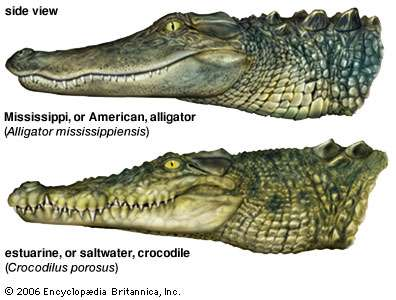
\includegraphics[scale=0.5]{crocodylia/alligatoridae/side.jpg}
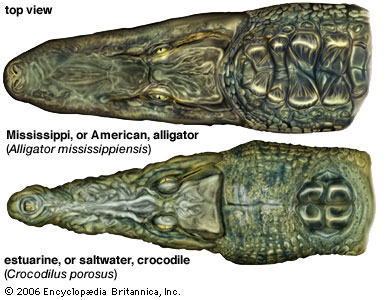
\includegraphics[scale=0.5]{crocodylia/alligatoridae/top.jpg}

\end{center}

\pagebreak
\section{Testudines}

\subsection{Chelydridae - Snapping Turtle}
\begin{center}
\begin{longtabu} to \textwidth {| | p{3.5cm} | X | |}

	\hline
	Taxonomy/Ancestry &
	7 extinct, 2 extant genera.
	
	\textbf{chelydra} -- 3 species native to the Americas
	
	\textbf{macrochelys} -- much larger alligator snapping turtle, 2 species exclusively N. American forming the largest freshwater turtles in N. America. A 3rd species has been proposed, the Apalachicola.
	\begin{itemize}[noitemsep]
		\item Most closely related to Platysternidae (big-headed turtles)
		\item Sometimes considered as subfamilies within the same family, but genetic evidence supports recognition as separate families
		\item Fossil record dating from Paleocene of N. America and Oligocene of Eurasia
		\item \emph{Chelydra} is known from as far back as the Pliocene in N. America
		\item \emph{Macrochelys} is known from as far as early Miocene
	\end{itemize}
	
	\begin{center} 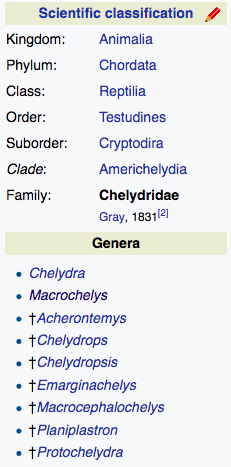
\includegraphics[scale=0.5]{testudines/chelydridae/tax} \end{center}
	 \\
	\hline
	Size & 
	7.1-31.5 in (18-80 cm); up to 249 lb (113 kg)
	\\
	\hline
	Color &
	
	 \\
	\hline
	Anatomy &
	\begin{itemize}[noitemsep]
		\item long tail
		\item 3 rows of tubercles*
		\item hooked beak
		\item kelled*, posteriorly separated carapace
		\item reduced, cruciform*, hingeless plastron
		\item heavy claws
		\item 11 marginal scutes on each side of the carapace
		\item abdominal scutes on plastron reduced; not in contact medially
		\item carapace and plastron connected by narrow bony bridge
		\item posterior skull roof deeply emancipated
	\end{itemize}
	
	The alligator snapping turtle is characterized by a large, heavy head, and a long, thick shell with three dorsal ridges of large scales (osteoderms), giving it a primitive appearance reminiscent of some of the plated dinosaurs, most notably the ankylosaurs. They can be immediately distinguished from the common snapping turtle by the three distinct rows of spikes and raised plates on the carapace, whereas the common snapping turtle has a smoother carapace. They are a solid gray, brown, black, or olive-green in color, and often covered with algae. They have radiating yellow patterns around their eyes, serving to break up the outline of the eyes to keep the turtle camouflaged. Their eyes are also surrounded by a star-shaped arrangement of fleshy, filamentous "eyelashes".
	 \\
	\hline
	Dimorphism & 
	males larger than females
	\\
	\hline
	Behavior & 
	\begin{itemize}[noitemsep]
		\item vicious temperament; since they are on top of the food chain, they have little fear
		\item snapping jaws used against prey and predators
		\item highly aquatic but leave water to nest or travel over land to reach new habitats or lay eggs
		\item diurnal, but nocturnal activity rare in northern populations
		\item most hibernate, but many individuals are capable of going w/o hibernation and remaining active beneath ice. Hibernating snapping turtles do not breathe for, in the northern part of their range, more than six months since ice covers their hibernating site. These turtles can get oxygen by pushing their head out of the mud and allowing gas exchange to take place through the membranes of their mouth and throat. This is known as extrapulmonary respiration. If they cannot get enough oxygen through this method they start to utilize anaerobic pathways, burning sugars and fats without the use of oxygen. The metabolic by-products from this process are acidic and create very undesirable side effects by spring, which are known as oxygen debt.
		\item In shallow waters, common snapping turtles may lie beneath a muddy bottom with only their heads exposed, stretching their long necks to the surface for an occasional breath (their nostrils are positioned on the very tip of the snout, effectively functioning as snorkels).
		\item Common snapping turtles sometimes bask---though rarely observed---by floating on the surface with only their carapaces exposed, though in the northern parts of their range, they also readily bask on fallen logs in early spring. 

	\end{itemize}
	\\
	\hline
	Habitat & 
	Common habitats are shallow ponds or streams. Some may inhabit brackish environments, such as estuaries. 
	\\
	\hline
	Distribution & 
	\textbf{common snapping turtle}: southeastern Canada, southwest to the edge of the Rocky Mountains, as far east as Nova Scotia and Florida.
	
	\textbf{alligator snapping turtle}: southeastern United States waters. They are found from the Florida Panhandle west to East Texas, north to southeastern Kansas, Missouri, southeastern Iowa, western Illinois, southern Wisconsin, southern Indiana, western Kentucky, and western Tennessee. They are found on the Missouri River at least as far north as the Gavins Point Dam, the southernmost dam on the Missouri River at Yankton, South Dakota, and are featured in the Gavins Point Dam Aquarium.
	
	Located from sea level to 2000 m elevation.
	\\
	\hline
	Feeding Ecology & 
	Snapping turtles consume both plant and animal matter, and are important aquatic scavengers, but they are also active hunters that prey on anything they can swallow, including many invertebrates, fish, frogs, reptiles (including snakes and smaller turtles), unwary birds, and small mammals. In some areas, adult snapping turtles can be incidentally detrimental to breeding waterfowl, as they will occasionally take ducklings and goslings but their effect on such prey is frequently exaggerated.
	
	Common snapping turtles have few predators when older, but eggs are subject to predation by crows, mink, skunks, foxes, and raccoons. As hatchlings and juveniles, most of the same predators will attack them as well as herons (mostly great blue herons), bitterns, hawks, owls, fishers, bullfrogs, large fish, and snakes. There are records during winter in Canada of hibernating adult common snapping turtles being ambushed and preyed on by northern river otters Other natural predators which have reportedly preyed on adults include coyotes, black bears, alligators and their larger cousins, alligator snapping turtles. Large, old male snapping turtles have very few natural threats due to their formidable size and defenses, and tend to have a very low annual mortality rate
	\\
	\hline
	Reproductive Biology & 
	 Courtship is variable and poorly developed and may include direct mounting, following of the female, face-offs/head-swaying, etc.
	 
	 This species mates from April through November, with their peak laying season in June and July. The female can hold sperm for several seasons, using it as necessary. Females travel over land to find sandy soil in which to lay their eggs, often some distance from the water. After digging a hole, the female typically deposits 25 to 80 hard-shelled, but not brittle eggs each year, guiding them into the nest with her hind feet and covering them with sand for incubation and protection. Incubation time is temperature-dependent, ranging from 9 to 18 weeks. In cooler climates, hatchlings overwinter in the nest. 
	 
	 TSD: intermediate temperatures produce male offspring, while high and low extremes produce females. clutches are so large that different areas of the nest may produce different sex ratios.
	 
	 Though their potential lifespans in the wild are unknown, alligator snapping turtles are believed to be capable of living to 200 years of age, but 80 to 120 is more likely. In captivity, they typically live between 20 and 70 years.
	\\
	\hline
	Ecological Role &
	have been seen as invasive species in Italy and Japan, as well as the Czech Republic and Germany for the alligator snapping turtle.
	\\
	\hline
	Conservation Status & 
	\textbf{common snapping turtle}: used as food w/ turtle soup. The species is currently classified as Least Concern by the IUCN, but has declined sufficiently due to pressure from collection for the pet trade and habitat degradation that Canada and several U.S. states have enacted or are proposing stricter conservation measures. In Canada, it is listed as 'Special Concern' in the Species at Risk Act in 2011 and is a target species for projects that include surveys, identification of major habitats, investigation and mitigation of threats, and education of the public including landowners. Involved bodies include governmental departments, universities, museums, and citizen science projects.

	\textbf{alligator snapping turtle}: Because of collection for the exotic pet trade, overharvesting for their meat, and habitat destruction, some states have imposed bans on collecting alligator snapping turtles from the wild. The IUCN lists it as a threatened species, and as of June 14, 2006, it was afforded some international protection by being listed as a CITES III species (which will put limits on exportation from the United States and all international trade in this species). The alligator snapping turtle is now endangered in several states, including Kentucky, Indiana, Illinois, and Missouri, where they are protected by state law. They are designated as ``in need of conservation" in Kansas.
	\\
	\hline
\end{longtabu}
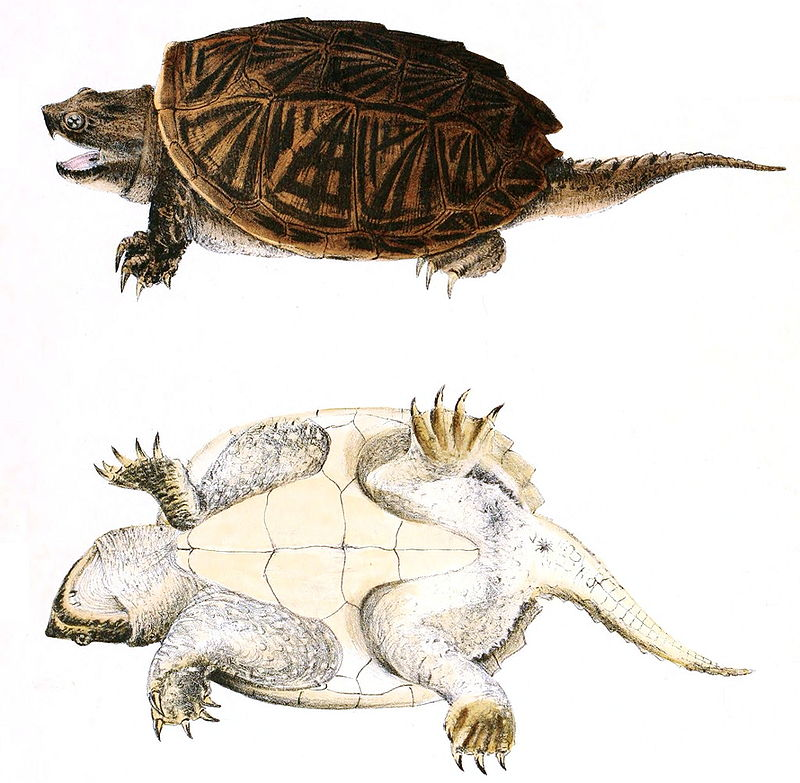
\includegraphics[scale=0.25]{testudines/chelydridae/common}
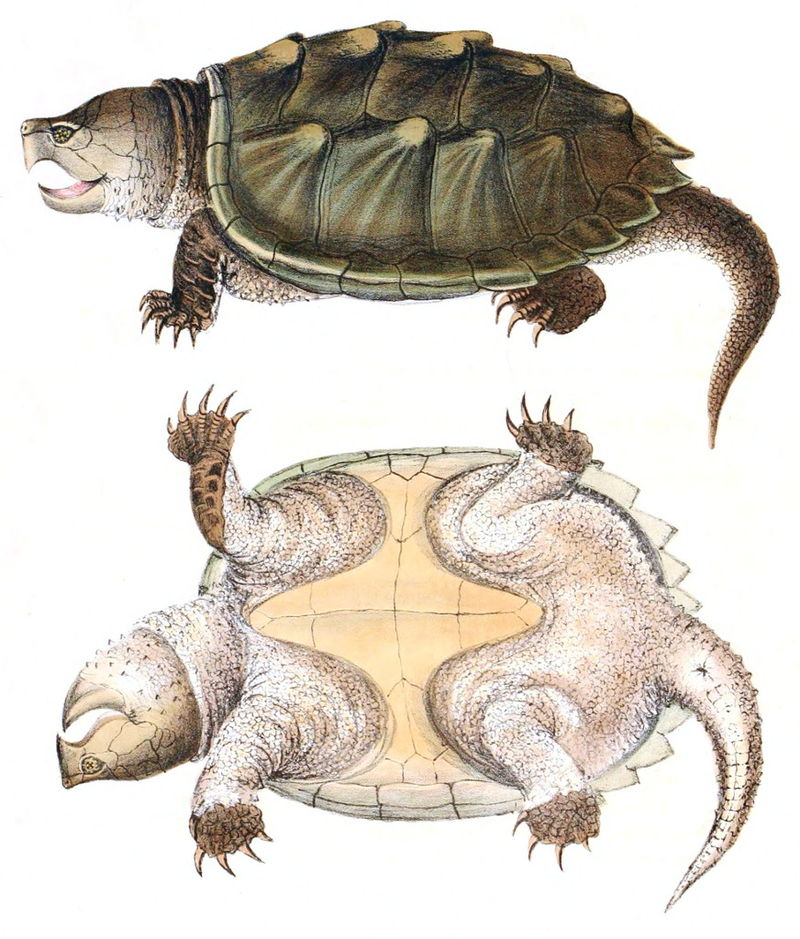
\includegraphics[scale=0.25]{testudines/chelydridae/alligator}
\end{center}
\pagebreak
\subsection{Kinosternidae --- Musk and Mud Turtles}
\begin{center}
\begin{longtabu} to \textwidth {| | p{3.5cm} | X | |}
	\hline
	Taxonomy/Ancestry &
	\begin{itemize}[noitemsep]
		\item 24 species within 4 genera, but taxonomic reclassification ongoing
		\item \emph{kinosternon} --- ``mud turtles," small aquatic turtles from the Americas
		\item \emph{sternotherus} --- ``musk turtles," endemic to N. America, closely related to \emph{kinosternon}
		\item \emph{claudius} --- only extant species is narrow-bridged musk turtle found in Mexico, Guatemala, and Belize
		\item \emph{staurotypus} --- Mexican musk turtles; giant musk turtles; three-kelled musk turtles; 2 recognized species found in Mexico and Central America
	\end{itemize}
	
	\begin{center} 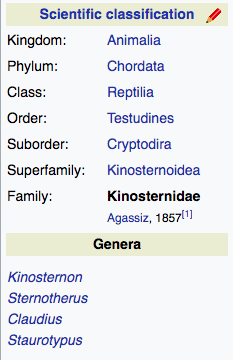
\includegraphics[scale=0.5]{testudines/kinosternidae/tax} \end{center}
	 \\
	\hline
	Size & 
	typically small, 10-15 cm (3.9-5.9 in) in length, but \emph{staurotypus} can get much larger, up to 30 cm (12 in).
	\\
	\hline
	Color &
	may be black, green, or yellowish in color. 
	
	most species don?t have shell markings, but some have radiating black markings on each carapace scute. some species have distinctive yellow striping along head and neck.
	 \\
	\hline
	Anatomy &
	\begin{itemize}[noitemsep]
		\item tall, highly domed upper carapace w/ distinct keel down center
		\item plastron differs by species
			\begin{itemize}[noitemsep] 
				\item some species have 1 or 2 hinges reaching from left to right side of shell; other species have none. the hinges allow plastron and carapace to pull tight against each other after the turtle pulls itself into the shell.
				\item some species have plastron covering only part of lower body; others have large plastron almost entirely concealing undersides
			\end{itemize}
		\item barbles* hanging from chin
		\item glands/sacs along side produce characteristic musky substance (smells like skunk spray)
	\end{itemize}
	 \\
	\hline
	Dimorphism & 
	Males usually have thicker and longer tails tipped w/ a spine; also have 2 rough, scaly patches on each leg. females are typically larger than males.
	\\
	\hline
	Behavior & 
	\begin{itemize}[noitemsep]
		\item aquatic for majority of lifespan
		\item slow swimmers
		\item travel to land for nesting or to feed during rainy season
		\item some diurnal, others nocturnal
		\item hibernation/estivation:
			\begin{itemize}[noitemsep]
				\item yellow mud turtle holds record for amt of time spent hibernating/estivating: inactive from winter to spring, summer to fall, only awakening when spring rains flood ground
				\item warm, wet climates --> active all year
				\item cold winters and deserts w/ long stretches of dry weather --> active only a few months a year and spend the rest underground waiting for better conditions
			\end{itemize}
		\end{itemize}
				
	\\
	\hline
	Habitat & 
	freshwater species living in still or slow-moving waters. prefer year-round bodies such as lakes or ponds. a few reside in shallow, seasonal ponds which have water only during a few months of the year, typically spring.
	\\
	\hline
	Distribution & 
	native to Americas
	\\
	\hline
	Feeding Ecology & 
	carnivorous turtles eating snails, clams, insects, worms, leeches, and sometimes freshly killed fishes they find. those w/ large heads typically prefer snails and clams which they can easily open w/ their jaws. in seasonal ponds, they may eat a large amount of seeds.
	\\
	\hline
	Reproductive Biology & 
	\begin{itemize}[noitemsep]
		\item no courtship rituals; mating takes place in water
		\item females go onto land to nest. they may either bury eggs in a hole they dig or simply lay eggs on surface leaves.
		\item lay 3-6 hard-shelled eggs during late spring and early summer
		\item up to 6 clutches per year
		\item oblong eggs range from 0.9-1.7 in (2.3-4.3 cm) long and from 0.6-1.0 in (1.5-2.5 cm) wide
		\item hatch 75 days to a year after being laid
		\item TSD: medium temperatures produce male offspring; females are produced by extremes
		\item post-eclosion, some species winter in subterranean nest and truly emerge in spring
		\item the yellow musk turtle is the only turtle species known to exhibit parental care. suggested to sometimes stay w/ nest and urinate on eggs long after laying to keep them moist or protect them from predators.
	\end{itemize}
	\\
	\hline
	Ecological Role &
	
	\\
	\hline
	Conservation Status & 
	4 VU; US Fish and Wildlife lists flatted musk turtle as Threatened. However, most species are quite common in their own habitats.
	\\
	\hline
\end{longtabu}
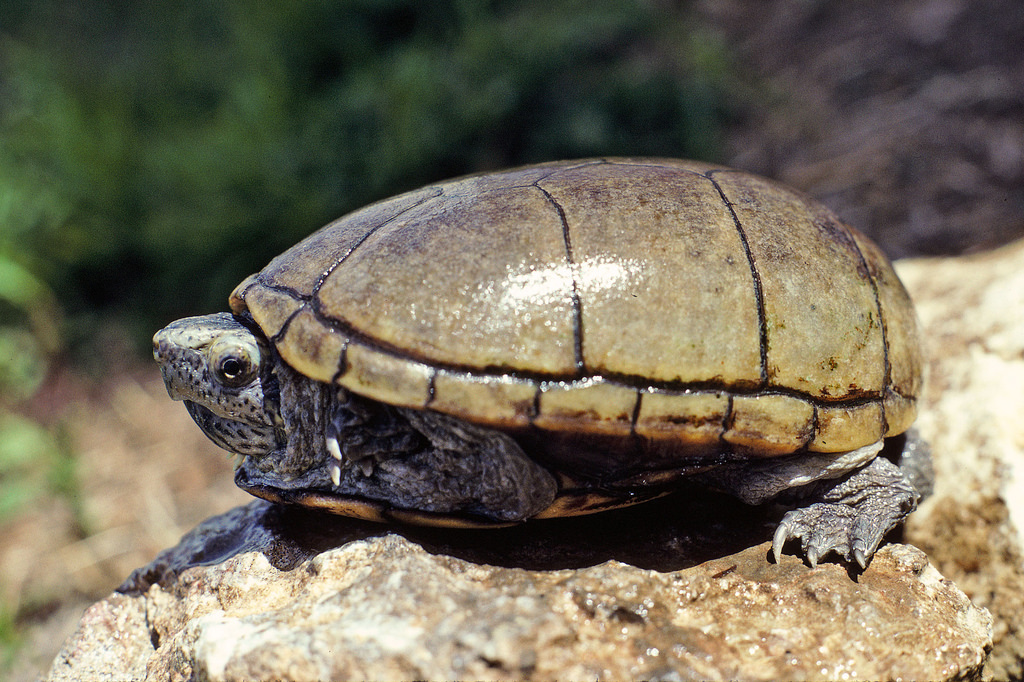
\includegraphics[scale=0.25]{testudines/kinosternidae/kino1}
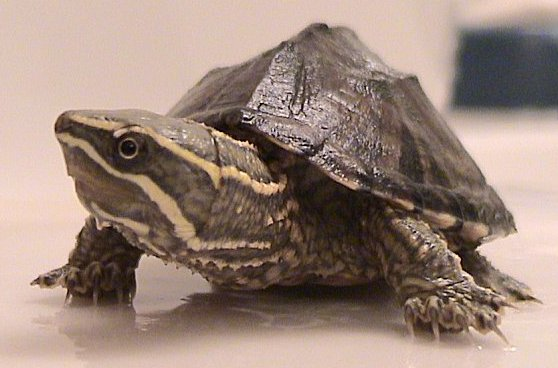
\includegraphics[scale=0.5]{testudines/kinosternidae/kino2}
\end{center}

\pagebreak
\subsection{Emydidae --- Box, Pond, and Marsh Turtles}
\begin{center}
\begin{longtabu} to \textwidth {| | p{3.5cm} | X | |}
	\hline
	Taxonomy/Ancestry &
	the largest and most diverse turtle family, w/ about 50 species in 10 genera. previously, several species of Asian box turtles were classified as Emydidae but now they have been moved to another family. it contains 2 subfamilies: Emydinae and Deirochelyinae.
	
	the oldest fossils are known from Upper Cretaceous and Paleocene of N. America. in modern times, closest relatives = Geoemydidae and Testudinidae (tortoises). as recognized today, Emydidae family includes primarily New World species.
	
	\begin{center} 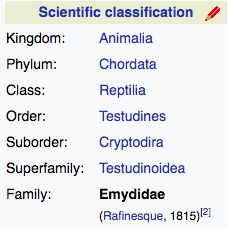
\includegraphics[scale=0.5]{testudines/emydidae/tax} \end{center}
	 \\
	\hline
	Size & 
	10-24 in (25-60 cm)
	\\
	\hline
	Color &
	
	 \\
	\hline
	Anatomy &
	\begin{itemize}[noitemsep]
		\item most diverse turtles in appearance
		\item the carapace typically takes the form of a low arch, but is domed in some
		\item some have keels* in the form of 1-2 ridges running from the front to the back
		\item a prominent bridge often connects the carapace to the plastron
		\item typically 8 pleugrals, 5 vertebrals, and 24 marginals on carapace
		\item 12 scutes on the plastron
		\item seam b/w posterior marginal scutes and last vertebral overlap pygal bone
		\item some members have moveable hinge separating pectoral and abdominal segments
		\item small skulls
		\item toe webbing
	\end{itemize}
	 \\
	\hline
	Dimorphism & 
	Males generally smaller than females in aquatic emydids, but this may be reversed among semiaquatic and terrestrial species.
	\\
	\hline
	Behavior & 
	\begin{itemize}[noitemsep]
		\item well-developed basking habit
		\item some active year-round; others seasonally inactive
			\begin{itemize}[noitemsep]
				\item in temperate northern species, hibernacula are generally located in well-oxygenated areas of water, but painted and Blanding's turtles are tolerant of hypoxic conditions
				\item at least 2 aquatic species, chicken turtle (Deirochelys reticularia) and western pond turtle known to hibernate terrestrially
				\item eastern box turtle  (Terrapene carolina) burrows beneath leaf litter and hibernates in shallow soil to survive subfreezing temps
			\end{itemize}
		\item elaborate courtship
	\end{itemize}
	\\
	\hline
	Habitat & 
	\begin{itemize}[noitemsep]
		\item Found in diverse range of habitats
		\item Occur abundantly in most permanent freshwater rivers, streams, lakes, and ponds
		\item One species found only in estuaries/coastal waters
		\item May be semi-aquatic to fully terrestrial
	\end{itemize}
	\\
	\hline
	Distribution & 
	\begin{itemize}[noitemsep]
		\item Found in lowland temperate regions of N. America, S. Africa, southern Turkey, Middle East, and throughout Europe to southern Russia
		\item Formerly more widespread in Europe but Scandinavian populations extirpated during Pleistocene
	\end{itemize}
	\\
	\hline
	Feeding Ecology & 
	\begin{itemize}[noitemsep]
		\item Includes diets from strictly herbivorous to strictly carnivorous
		\item Hatchlings of many species highly carnivorous, but become omnivorous as they mature
		\item Some have diverse, generalized diets; others have highly specialized diets
		\item Map turtle (genus Graptemys) females may be develop huge heads w/ broad palates to crush large mollusks
		\item Chicken turtles and Blanding?s turtles independently evolved long neck w/ well-developed hyoid apparatus (elaborate bony structure that rapidly expands throat to suck in prey items)
		\item Hyoid apparatus commonly found in piscivorous turtle species
	\end{itemize}
	\\
	\hline
	Reproductive Biology & 
	\begin{itemize}[noitemsep]
		\item mating generally occurs in the spring, but some species may store sperm from earlier matings for many years
		\item many species display elaborate courtship utilizing thin forelimb claws which are vigorously waved at females; a unique pattern of head bobs may be exchanged
		\item the female allows the male to mate, suggesting the females choose whom to mate with
		\item elongated eggs may be flexible or brittle-shelled
		\item most exhibit TSD
	\end{itemize}
	\\
	\hline
	Ecological Role &
	
	\\
	\hline
	Conservation Status & 
	\begin{itemize}[noitemsep]
		\item 7 VU; 6 EN; 14 NT
		\item Human activities (eg pollution, habitat destruction, road mortality, and collection for pet trade) responsible for most species? decline
		\item Ex --- Diamondback terrapin (Malaclemys terrapin) once faced extinction due to overcollection for human consumption, but recovered as it fell out of favor w/ wealthy ppl
	\end{itemize}
	\\
	\hline
\end{longtabu}
\end{center}
\subsubsection{Terrapene --- Box Turtles}
\begin{center}
\begin{longtabu} to \textwidth {| | p{3.5cm} | X | |}

	\hline
	Taxonomy/Ancestry &
	a member of the subfamily emydinae. 12 taxa over 4 species. Terrapene originally coined as genus separate from Emys for species w/ sternun separated into 2-3 divisions which can move independently.
	
	they appear abruptly in the fossil record in modern form, implying they are a generalist species able to survive under a wide variety of conditions. older fossils have been found in Nebraska dating back to the Miocene (15 Mya). only recognized extinct subspecies dates from Pliocene and was much larger than other species.
	
	\begin{center} 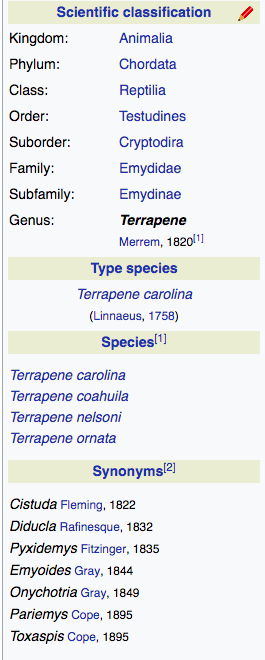
\includegraphics[scale=0.25]{testudines/emydidae/terrapene/tax} \end{center}
	 \\
	\hline
	Size & 
	10-22cm (4-9 in)
	\\
	\hline
	Color &
	females usually have yellowish-brown eyes, while males typically have red or orange eyes.
	 \\
	\hline
	Anatomy &
	\begin{itemize}[noitemsep]
		\item distinguished by domed shell which is hinged at the bottom
			\begin{itemize}[noitemsep]
				\item allows animal to close shell tightly to escape predators
			\end{itemize}
		\item item avg. lifespan of 50 yrs, but many can live past 100. once maturity is reached, the chances of death do not seem to increase w/ age.
		\item age can be roughly estimated by counting growth rings on scutes, but estimates may be inaccurate b/c the plastron is worn smooth over time.
	\end{itemize}
	 \\
	\hline
	Dimorphism & 
	Males have concave area on plastron centered beneath hinge.
	\\
	\hline
	Behavior & 
	\begin{itemize}[noitemsep]
		\item defend selves from predation by hiding, closing shell, and biting, but are vulnerable to surprise attacks and persistent gnawing/pecking
		\item tend to move further into woods prior to hibernation
	\end{itemize}
	\\
	\hline
	Habitat & 
	\begin{itemize}[noitemsep]
		\item no standard habitat, but generally found in mesic woodlands
		\item \emph{T. ornata} can be found in grasslands
		\item desert box turtle can also be found in semidesert w/ rainfall predominantly in summer
		\item Coahuilan box turtles found only in region characterized by marshes, permanent presence of water, and cacti
	\end{itemize}
	\\
	\hline
	Distribution & 
	native to N. America, where the species w/ the widest range, the common box turtle, is found in the US and Mexico. the ornate box turtle is endemic to south-central and southwestern US/adjacent Mexico, the spotted box turtle is endemic to northwestern Mexico, and the Coahuilan box turtle found only in Cuatro Cienegas Basin in Coahuila, Mexico.
	\\
	\hline
	Feeding Ecology & 
	an omnivore w/ a varied diet, it eats anything it can catch. invertebrates/insects = principal component but diet also consists of vegetation. the diet can be amended w/ fruits. at times, it eats poisonous mushrooms, making its meat dangerous for humans.
	\\
	\hline
	Reproductive Biology & 
	relatively slow reproducers, they reach sexual maturity only after 4-5 yrs. females can store viable sperm in the oviducts for up to 4 yrs. they mate from may-october and lay elliptical, leathery eggs in flask-shaped holes 3-4 in deep in warm, sunny soil. they may have more than 1 clutch a yr, w/ avg. clutch size being larger in northern populations and ranging from 1-7 eggs. incubation takes 2-3 months. infant mortality is high, since the shell is weaker. infants may overwinter in the nest.
	\\
	\hline
	Ecological Role &
	
	\\
	\hline
	Conservation Status & 
	\begin{itemize}[noitemsep]
	\item 1 EN; 1 V; 1 NT; 1 DD
	\item Often taken as or bred as pets
		\begin{itemize}[noitemsep]
			\item Easily stressed and require more care than is generally thought
			\item Require outdoor enclosure and constant exposure to sun
			\item Recommended to buy captive bred to reduce pressure on wild populations
		\end{itemize}
	\item Some states prohibit collecting wild turtles or require permits to keep them
	\item State reptile of N. Carolina, Tennessee, Missouri, and Kansas
	\end{itemize}
	\\
	\hline
\end{longtabu}
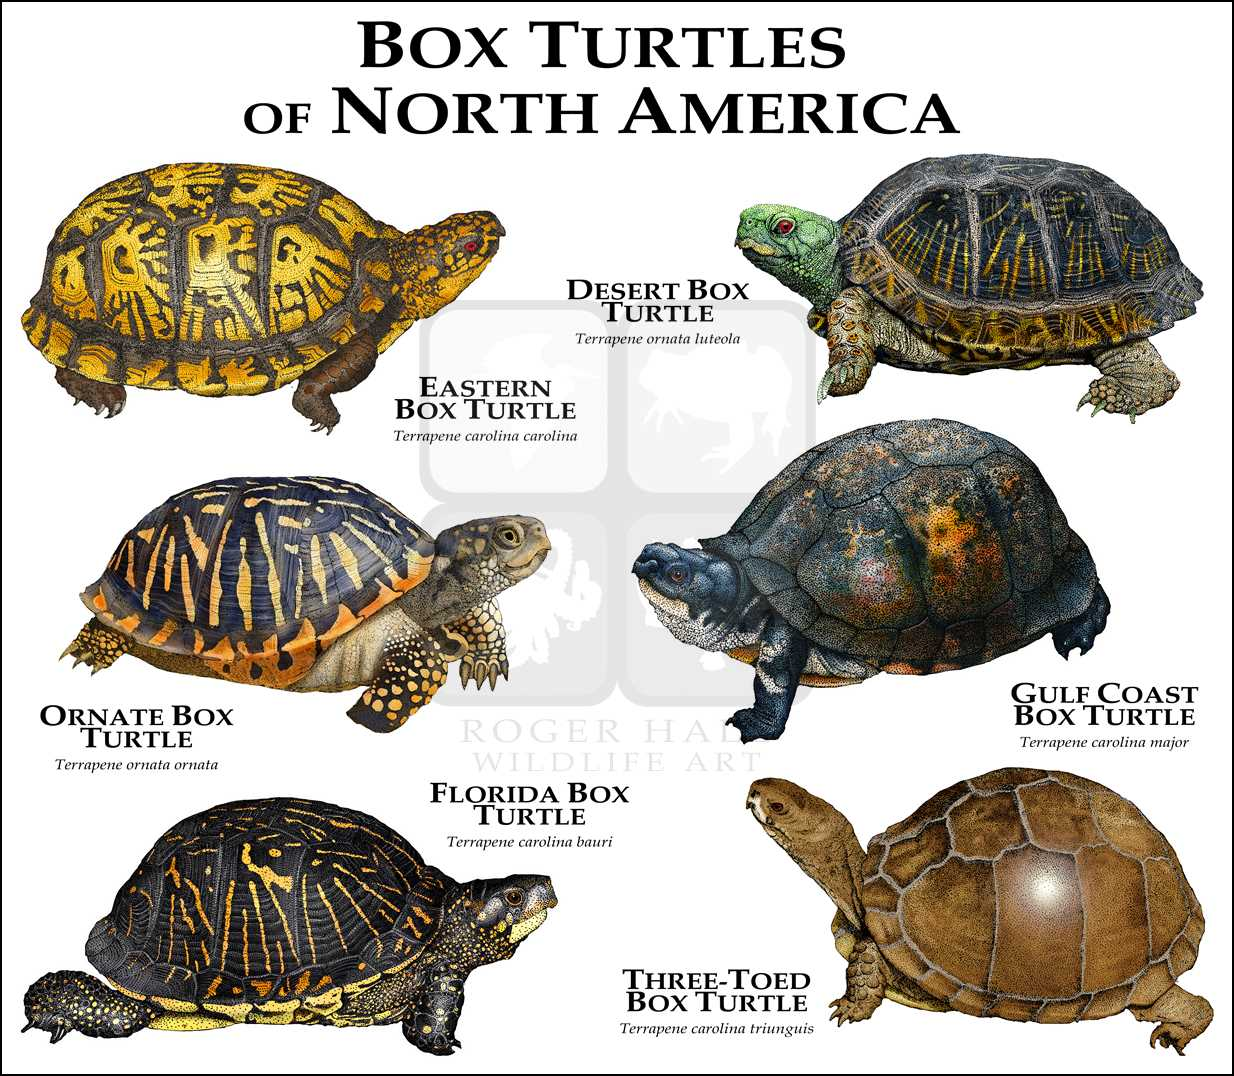
\includegraphics{testudines/emydidae/terrapene/box}
\end{center}
\end{document}

%glossary: barbels, estivation, keels, shell anatomy (see emydidae), scutes, hibernacula, hyoid apparatus, state reptiles.